\documentclass{article} %document style and layout
\usepackage{enumitem} %list of elements
\usepackage{imakeidx}
\usepackage{hyperref}
\usepackage{xcolor}
\usepackage{graphicx}
\usepackage{subcaption}
% \usepackage[utf8]{inputenc}
% \usepackage[T1]{fontenc}
\usepackage{listings} %package to import code
\lstdefinestyle{mystyle}{
    backgroundcolor=\color{backcolour},   
    commentstyle=\color{code_green},
    keywordstyle=\color{url_blue},
    stringstyle=\color{orange},
    basicstyle=\ttfamily\footnotesize,
    breakatwhitespace=false,         
    breaklines=true,                 
    captionpos=b,                    
    keepspaces=true,                 
    numbers=left,                    
    numbersep=5pt,                  
    showspaces=false,                
    showstringspaces=false,
    showtabs=false,                  
    tabsize=2
}
\lstset{style=mystyle}

\usepackage{titling}
\renewcommand\maketitlehooka{\null\mbox{}\vfill}
\renewcommand\maketitlehookd{\vfill\null}

%-------Titlepage information------------------------------------------
\title{\textbf{\huge{Wireless communications - Adaptive beamforming}}}
\author{Luca Ferraro (10748116), Bernardo Camajori Tedeschini (10584438), \\
            William Colombo (10537311)\\ 
\textcolor{url_blue}{\url{https://github.com/BernardoCama/WirelessCommunicationProject}}}
\date{A.Y. 2020/2021♯}
%----------------------------------------------------------------------

\begin{document}
\definecolor{url_blue}{rgb}{0,0.427,0.639} %rgb: 0, 109, 163 
\definecolor{backcolour}{rgb}{0.95,0.95,0.92}
\definecolor{code_green}{RGB}{11,102,35}

\begin{titlingpage}
    \maketitle
\end{titlingpage}

\newpage{}

\tableofcontents
\listoffigures
\lstlistoflistings
\newpage{}

%------------------------------------------------------------------------------------------------------------------------------------------------
\clearpage
\section{Introduction}
\label{sect:introduction}
In this section, we describe briefly the key concepts that 
are mandatory for the comprehension of the project.

\subsection{OFDM signal}

OFDM (Orthogonal Frequency Division Multiplexing)
is a multi-carrier modulation whose key feautures are:
\begin{enumerate}
    \item \textbf{Flexibilty} By means of:
    \begin{itemize}
        \item   \textbf{Adaptive Bit Loading} Adaptive modulation, coding for each sub-carrier.
        \item   \textbf{Multiple Access} Multiple Access Feature with the use of OFDMA.
    \end{itemize}
    \item \textbf{Digital Implementation} With the use of DFT and IDFT at Tx and Rx side respectively to pass from Samples in frequency domain to time domain and viceversa.
    \item \textbf{Simple Equalization} Through the use of Cyclic Prefix that permits the representation of the channel with a single tap (Flat Ch) in each sub-carrier.
    \item \textbf{MIMO Implemetaion} Suited for the use of MIMO/MMIMO Systems.
\end{enumerate}

The main parameters of the Modulation are:
\begin{enumerate}
    \item \textbf{Nsc} Number of sub-carrier which usually is in the form $2^{b}$ since it is optimized for the FFT and IFFT implementaion.\\
                        In our case: Nsc = 64.
    \item \textbf{CyclicPrefixLength} The length of Cyclic Prefix that must be much smaller than Ts (OFDM Symbol Time).\\
                        In our case: CyclicPrefixLength = 4.
    \item \textbf{NumGuardBandCarriers} The number of Guard Bands in frequency domain to protect the OFDM Spectrum from other adjacent trasmissions.\\
                        In our case: NumGuardBandCarriers = [1;1] one for each side.
    \item \textbf{Pilot Positions} The sub-carrier location of Pilot signals, known sequence of symbols that are used to estimate tha channel.\\
                        In our case: Pilotindices = [2]. We really don't use use the Pilot, since we consider the first symbols of the transmission as known, but for completeness we dropped off at least one Pilot.
\end{enumerate}


\subsection{3GPP Standard}

3GPP (3rd Generation Partnership Project) was founded in December 1998 when the European 
Telecommunications Standards Institute (ETSI) 
partnered with other standard development organizations (SDOs) 
from around the world to develop new technologies (technology specifications).

As Channel Model we use QuaDRiGa (QUAsi Deterministic RadIo channel GenerAtor) that 
generates realistic radio channel impulse responses for system-level simulations of mobile radio networks. 
Quadriga indeed is able to simulate 3GPP channel models like 3GPP-3D and also the latest New Radio channel model.


\subsection{Beamforming}

A beamformer can be considered a spatial filter that suppresses
the signal from all directions, except the desired ones by means 
of weights applied to the signals coming from the single array elements;
resulting in controlling the radiation pattern of the array.

The \textbf{Array Pattern Function} $AF(\theta,\phi)$ is the gain that we can obtain with the 
Beamformer in a given direction specified by:

\begin{itemize}
    \item $\theta$ = Elevation ($\pi/2$ - zenith of arrival)
    \item $\phi$ = AoA (angle of arrival)
\end{itemize}

and it is defined as: \\\\
$AF(\theta,\phi)$ = $w^Hs$ where:
\begin{itemize}
    \item $s$ are the Steering Vectors
    \item $w$ are the weigths of the Beamformer
\end{itemize}

In the project, in particular in \hyperref[sec:antenna_array_comparison]{section 4}, we compare the different \textbf{Array Pattern Function} 
of various type of Beamformer.


%------------------------------------------------------------------------------------------------------------------------------------------------
\clearpage
\section{Project description}
\label{sect:project}
In this section, we describe the structure of out project with a brief description of 
the main points of all the parts composing our work.

\subsection{Beamforming techniques}

We have implemented 5 beamforming techniques:

\begin{enumerate}
    \item \textbf{Simple beamforming} The phases are selected to steer the array in a particular direction.
    \item \textbf{Null-steering beamforming} Used to cancel K <= N-2 plane waves arriving from known directions.
    \item \textbf{Minimun variance distiortionless response (MVDR) beamforming} This beamformer minimizes the interference-plus-
            noise power at the output of the beamformer. 
    \item \textbf{Minimum mean square error (MMSE) beamforming} The weigths of the antennas are adjusted in a way that the
            MSE between the output of the beamformer and the reference signal is minimized.
    \item \textbf{Least mean square (LMS) beamforming} This iterative algorithms adjust the weights by estimating the
            gradient of the MSE and moving them in the negative direction of the gradient at each iteration. We have 
            implemented this iterative algorithm both in the time and in the frequency domain.
\end{enumerate}

\subsection{Channels}

All the 5 beamformers have been tested on 3 different channel:

\begin{enumerate}
    \item \textbf{LOS channel} A simple line of sigth channel with no reflections.
    \item \textbf{Two-ray channel} For each signal, we consider a direct path (LOS) and a single reflection.
    \item \textbf{Quadriga channel} Here, the scenario we have used is the \textit{QuaDRiGa\_UD2D\_LOS}.
\end{enumerate}

\subsection{Signals}

For all the beamformers and in all the channel, the bits we transmit are generated randomly and modulated fist with a 4\-QAM 
modulation (we have also tested the beamformers with a 16\-QAM); then, the QAM symbols are modulated with OFDM for transmission.

\subsection{Reported results}

In this report, we only describe the three most important simulations we have done:

\begin{enumerate}
    \item Comparison between the SNR at the input and at the output of all the five beamformers in a LOS channel (\hyperref[sec:snr_comparison]{section 3}).
    \item Comparison of the performance in terms of constellations revealed, weigths of the antennas and BER for all the \\ 
            five beamformers considering different antenna arrays (\hyperref[sec:antenna_array_comparison]{section 4}). This has been done in the quadriga channel \\ 
            and using the LMS beamformer in the time domain.
    \item Traking of a vehicle using LMS beamforming in the frequency domain (\hyperref[sec:tracking]{section 5}).
\end{enumerate}

All the other simulations we have done can be found on the \textit{Github} repository of the project (link in title page).


%------------------------------------------------------------------------------------------------------------------------------------------------
\clearpage
\section{SNR comparison}
\label{sect:project}
In this simulation, we have tested the performance in terms of gain in the SNR at the output of the five
 beamformers we have implemented for:

\begin{enumerate}
    \item Different number of interfering signals
    \item Different values of SNRs at the input of the beamformers
\end{enumerate}

\subsection{Geometry and parameters}

We are using a $LOS$ channel in stationary conditions (vehicles are not moving). The vehicles are positioned at a 
distance of 25 meters from the base station on a circumference and spaced of $20°$ as in Figure \ref{fig:Scenario_circle}. \\ 
The antenna array we are using is a 4x4 array.

\begin{figure}[ht]
    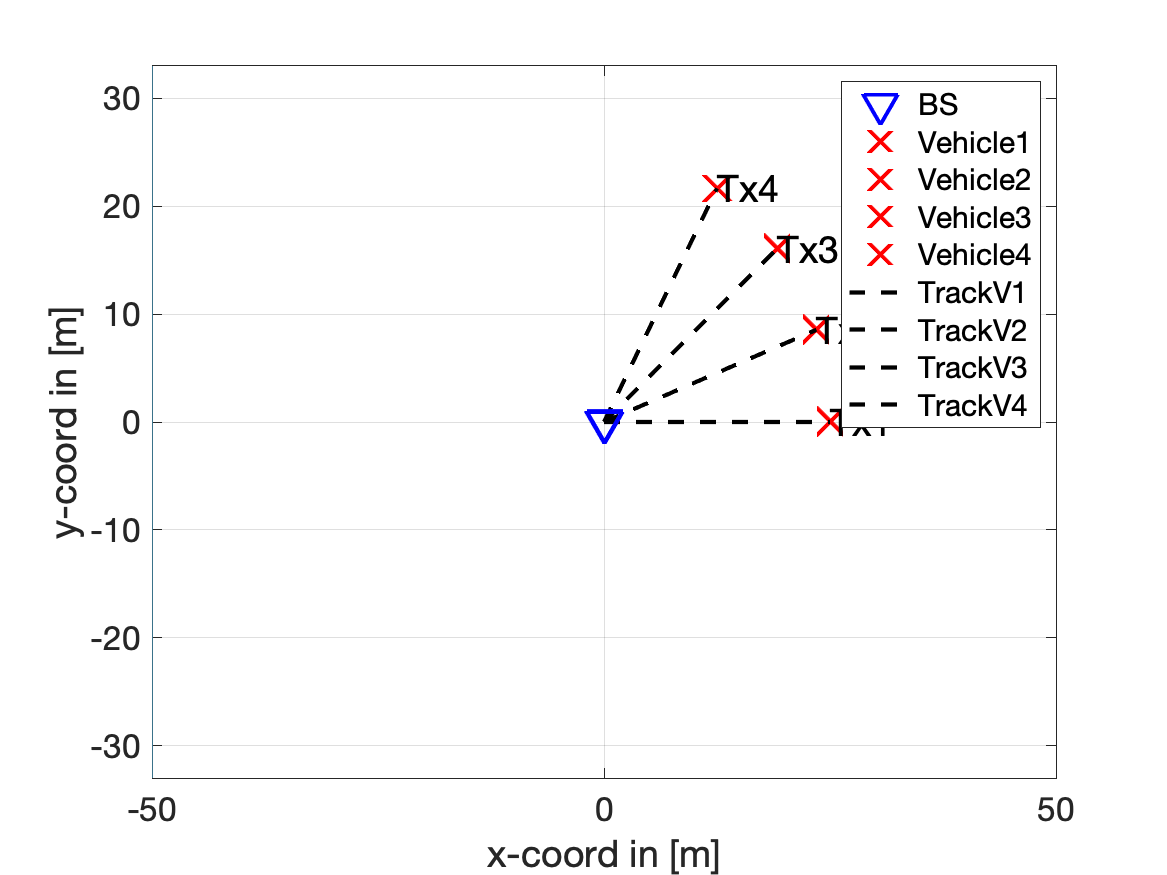
\includegraphics[width=\linewidth]{Scenario_circle.png}
    \caption{Scenario of the simulation}
    \label{fig:Scenario_circle}
\end{figure}

\subsection{Steps of the simulation}

Our simulation considers a different number of interferents (0, 1, 2, 3) and for each one of the cases computes the 
curve input SNR - output SNR for all the beamformers:

\begin{enumerate}
    \item Definition of the current number of interferents
    \item Generation of scenario and of singnals
    \item Passage of signals though the $LOS$ channel
    \item For all the input SNR levels:
    \begin{enumerate}
        \item Add noise to the good signal in a way that the SNR is the current one
        \item Computation of the weights of the antenna elements 
        \item Application of beamforming techniques to the single signals and noise
        \item Computation of the power of all the signals and of the noise
        \item Computation of the SNR at the output of the beamformers
    \end{enumerate}
    \item Plot of the results
\end{enumerate}

\subsection{Results}

In Figure \ref{fig:SNR_comparison}, we can see in the four graphs the curves SNRin - SNRout for the different
beamformers.

\begin{figure}[ht]
    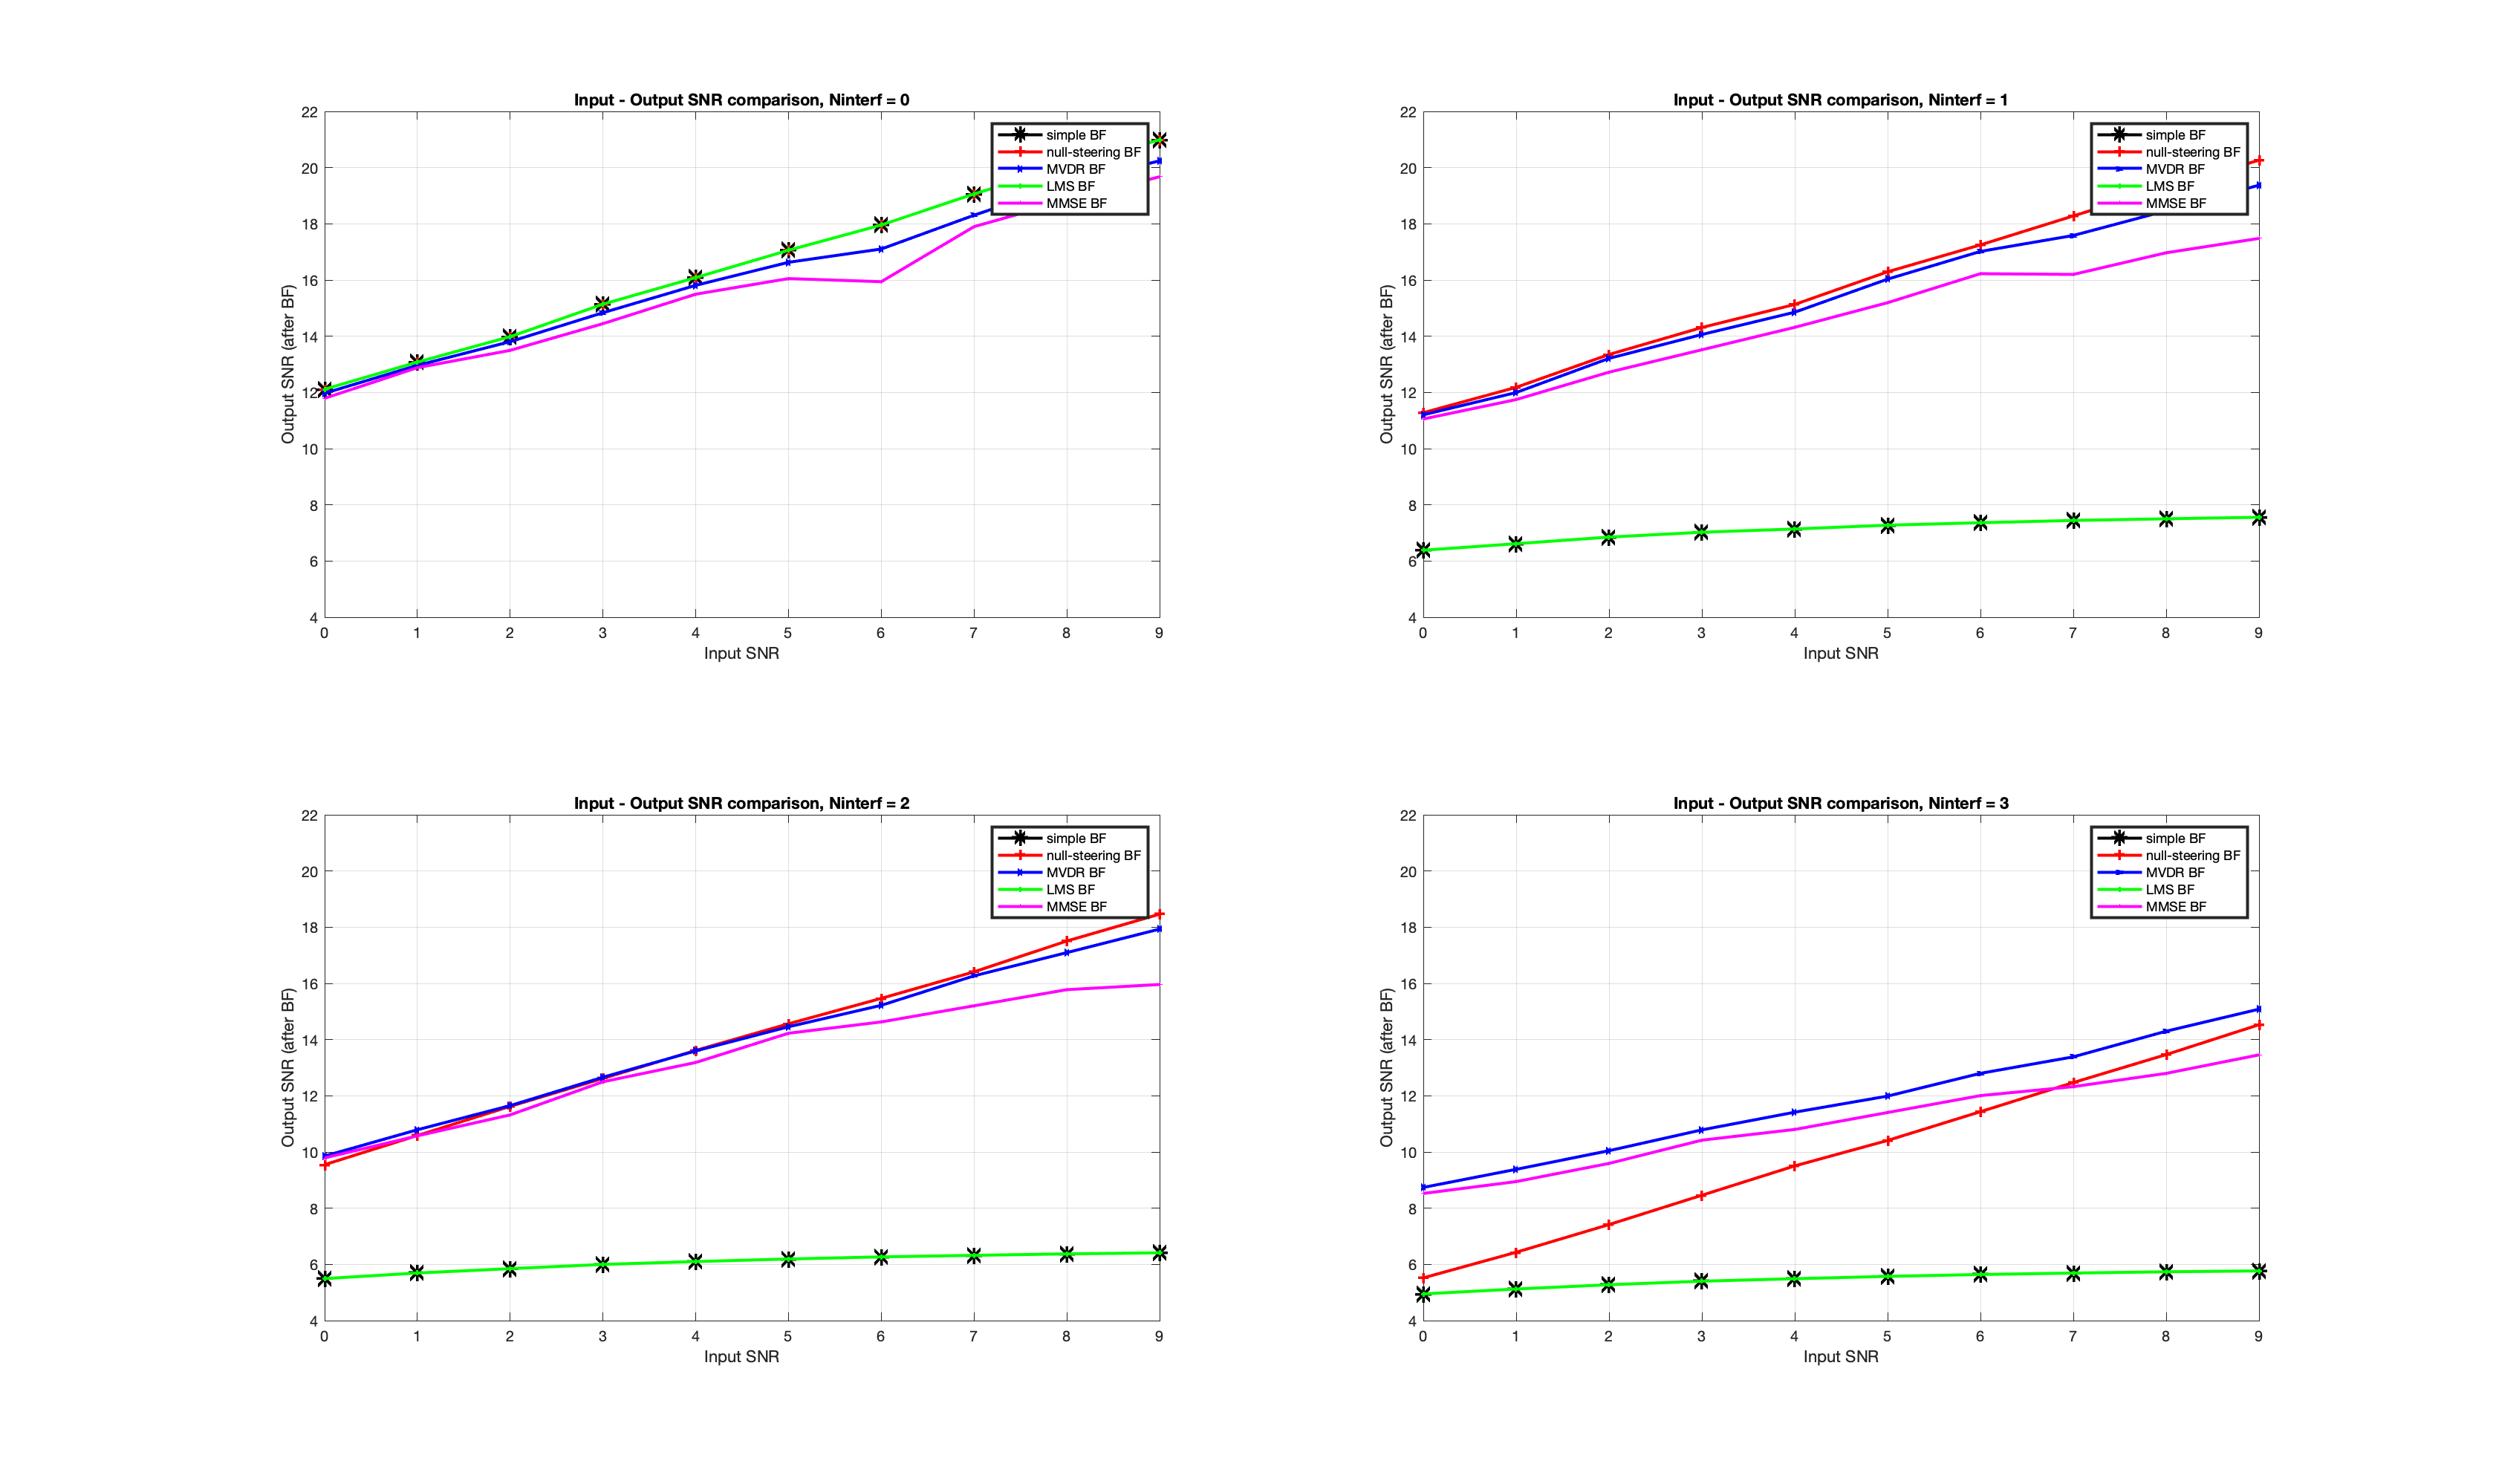
\includegraphics[width=\linewidth]{SNR_comparison.png}  
    \caption{Relation SNRin - SNRout for different interfering signals anf beamformers}  
    \label{fig:SNR_comparison}
\end{figure}

As we can see, without any interfering signals, the behavior of all the beamformers is almost linear and the gain is 
approximately constant and equal to 12dB.
As the number of interferents increases, we can identify as general behavior:

\begin{enumerate}
    \item The simple and the LMS beamformer is the worst one; indeed, their curves are the most bended and the 
            ones giving the lowest gain. This is expected for the simple beamformer and, in this case, also for the LMS
            since we are initializing its state using the simple beamformer. This is not the best way to initialize it (and
            in fact the gain of the LMS is low), but its a simple way of initializing it.
    \item 
\end{enumerate}

%------------------------------------------------------------------------------------------------------------------------------------------------
\clearpage
\section{Antenna array comparison}
\label{sect:project}
In this part of our project, we have compared the performance of the five beamforming techniques using different antenna arrays,
in particular we have used as arrays:

\begin{enumerate}
    \item 2x2
    \item 4x4
    \item 8x8
    \item 16x16
\end{enumerate}

\subsection{Aim of the experiment}

The aim of this experiment is to evaluate the performance of different beamforming techniques using different antenna arrays. In 
particular, for each beamformer and for each antenna array, we have studied:

\begin{enumerate}
    \item The shape of the $QAM$ constellation revealed. 
    \item The shape of the array pattern function.
    \item The $BER$
\end{enumerate}

\subsection{Geometry and parameters}

In this simulation, we have considered two sources that we call $V1$ and $V2$: the signal we want to receive is the one from $V1$,
while $V2$ is producing an interfering signal.\\ 
Both the vehicles are not moving and they are transmitting 100 $4\-QAM$ symbols.\\
The geometry of the symulation can be seen in Figure \ref{fig:Scenario_still}.

\begin{figure}[ht]
    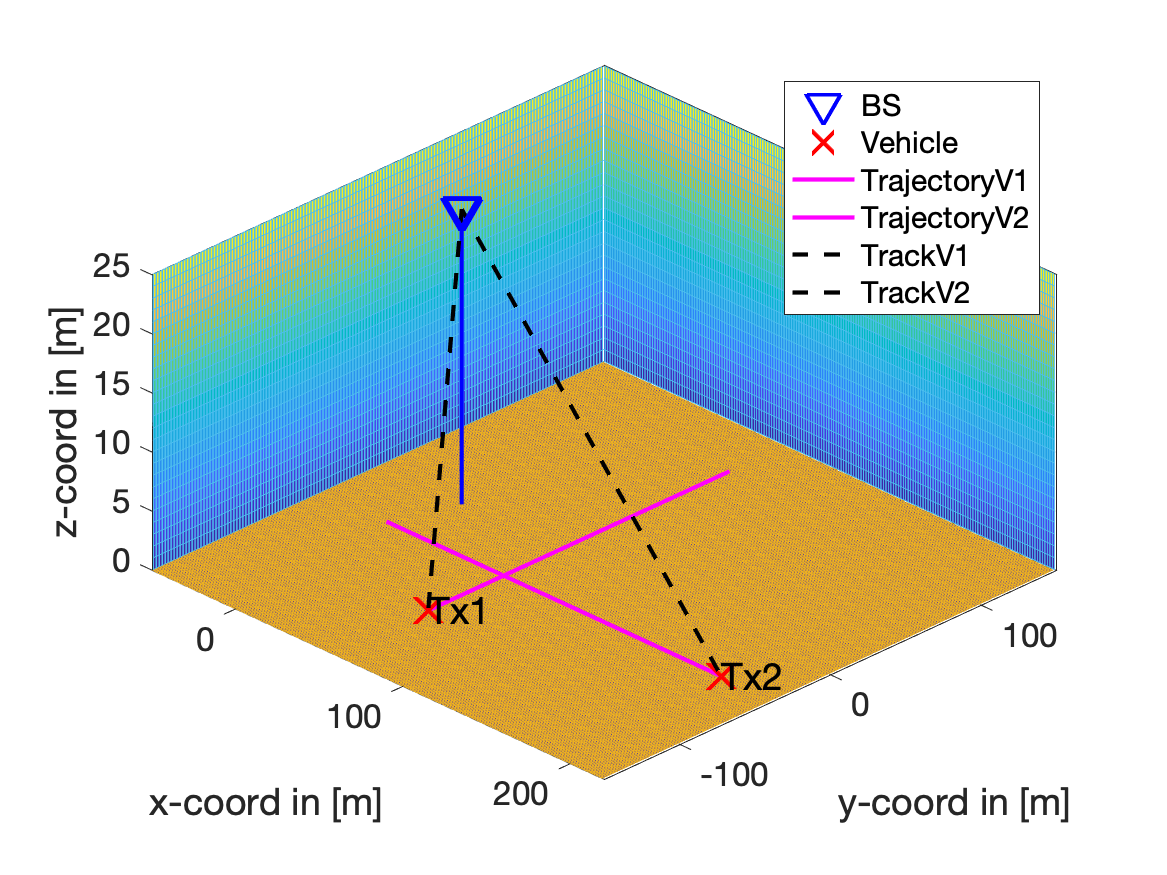
\includegraphics[width=\linewidth]{Quadriga1.png}
    \caption{Scenario of the simulation}
    \label{fig:Scenario_still}
\end{figure}

\subsection{Steps of the simulation}

The very first thing we do in our simulation is defining the geometry of our scenario, so positioning the vehicles and the base station.\\
Then, we prepare the signal to be transmitted, that is an OFDM signal modulating symbols from a 4\-QAM modulation.\\
The simulation proceeds with a loop on the four different antenna arrays. In each loop, the main steps we follow are:

\begin{enumerate}
    \item Definition of the current antenna array.
    \item Passage of the signal through the QuaDRiGa channel ()$QuaDRiGa\_UD2D\_LOS$ scenario).
    \item Estimation of the \textit{DoA} of the two vehicles using the \textit{MUSIC} algorithm.
    \item Application of the five beamformers to the received signal. Here, we use the real $DoA$, and not the estimated one
            for a more consistent comparison of the results.
    \item Channel equalization using the gradient descent algorithm. Here, we use a two-tap equalizer even if we could use only one 
            (since on each subcarrier of the OFDM signal we can consider the channel as flat) for being more precise.
    \item OFDM demodulation.
    \item QAM demodulation.
    \item Computation of the BER.
\end{enumerate}

At the end of the loop, we show the results by making some plots and videos that are commented below in the following sections.

\subsection{Results: \textit{QAM} constellations}

In the Figure \ref{fig:Constellations} we can see 4 images, one per antenna array; in each one of them, we have
plotted the constellation revealed by using the five different beamformers. \\ 
As we can see, in general the higher the number of antenna we are using, the more precise is the $QAM$ constellation. This
is due to the fact that with more antenna the precision in the angular localization of the source is more precise; therefore, 
the beam that points towards it is narrower and the interfering signal is more attenuated (this can be seen even better by
looking at the antenna pattern functions).

\begin{figure}[ht]
    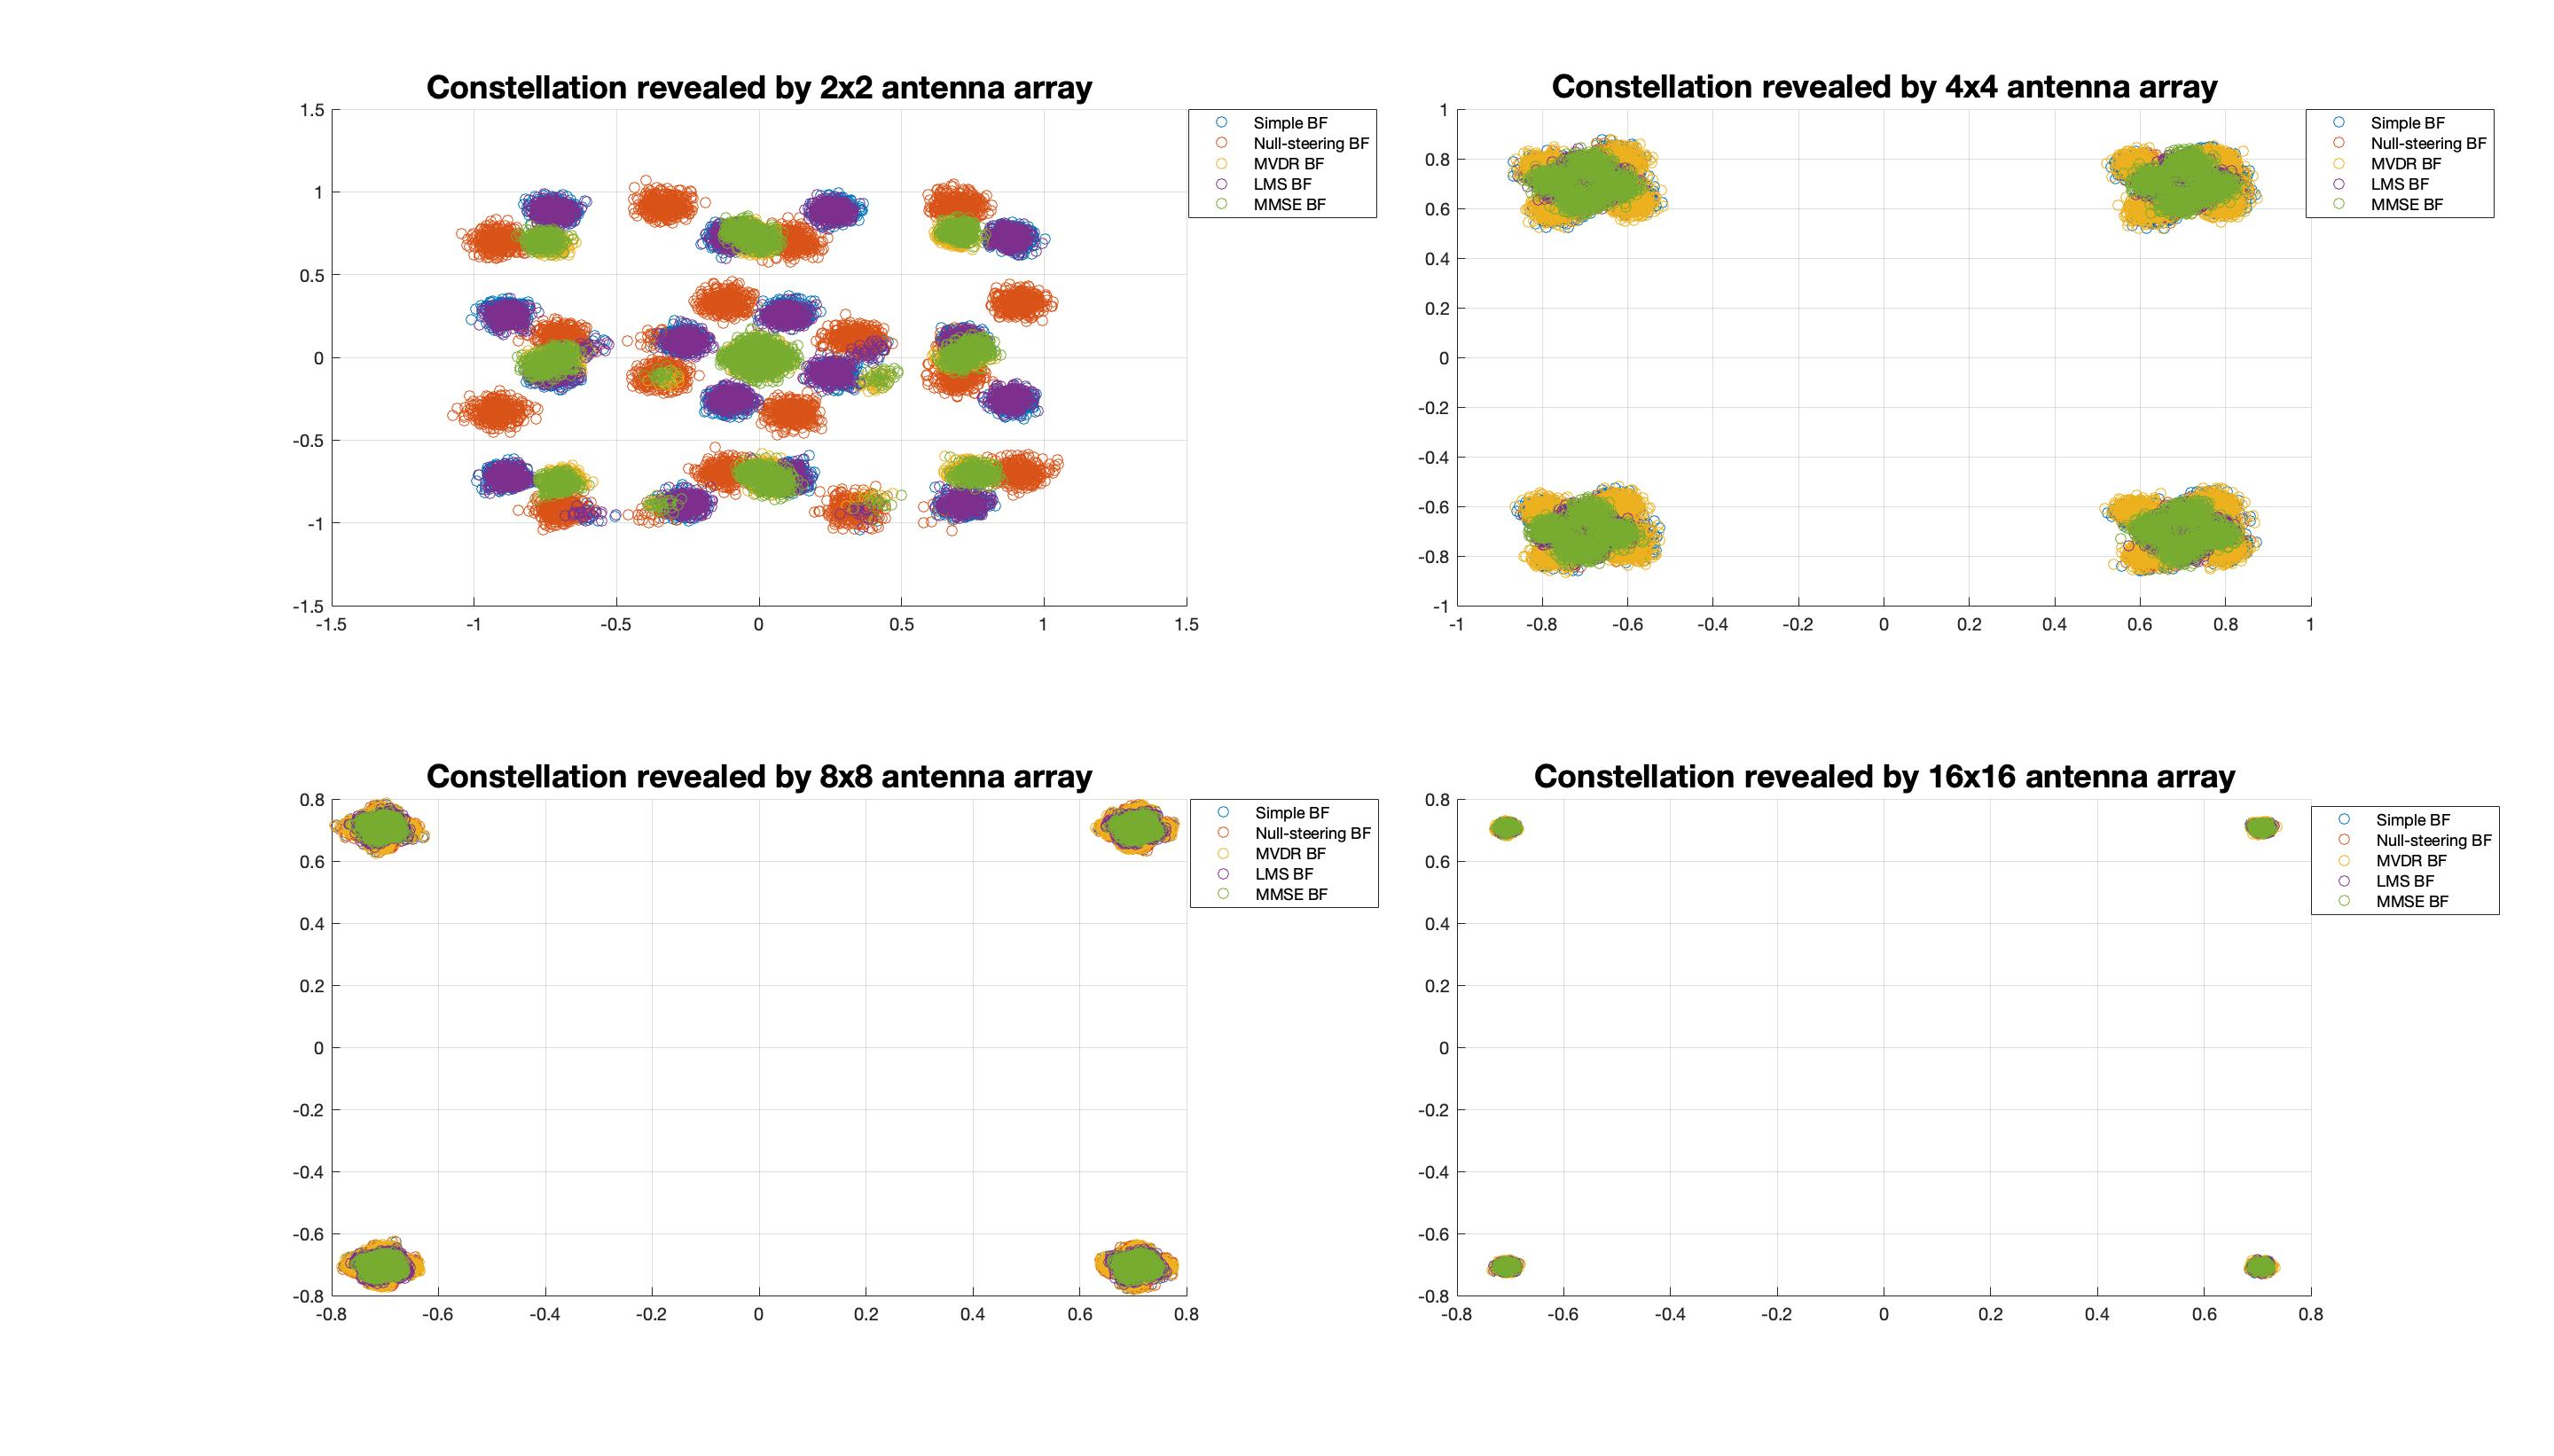
\includegraphics[width=\linewidth]{Constellations.jpg}
    \caption{4-QAM constellations}
    \label{fig:Constellations}
\end{figure}

\subsection{Results: antenna pattern functions}

The Figure \ref{{fig:Array_pattern} shows for each of the four antenna arrays the array pattern function of the five
beamforming techniques we have implemented; the array pattern functions have been plotted on the zenith angles of the source.
We have also plotted a vertical line that represents the $DoA$ of the source.\\
The most interesting things to be noticed are two:

\begin{enumerate}
    \item The maximum of all the antenna array pattern functions is always localized in correspondence of the $DoA$ of the source.
            This is indeed the aim of beamforming.
    \item The higher the number of antennas, the narrower the beam that is pointing in the direction of the source. This is due 
            to the fact that with more antenna we have more spatial samples of the signal and therefore a better estimation of 
            its angular positions. 
\end{enumerate}

\begin{figure}[ht]
    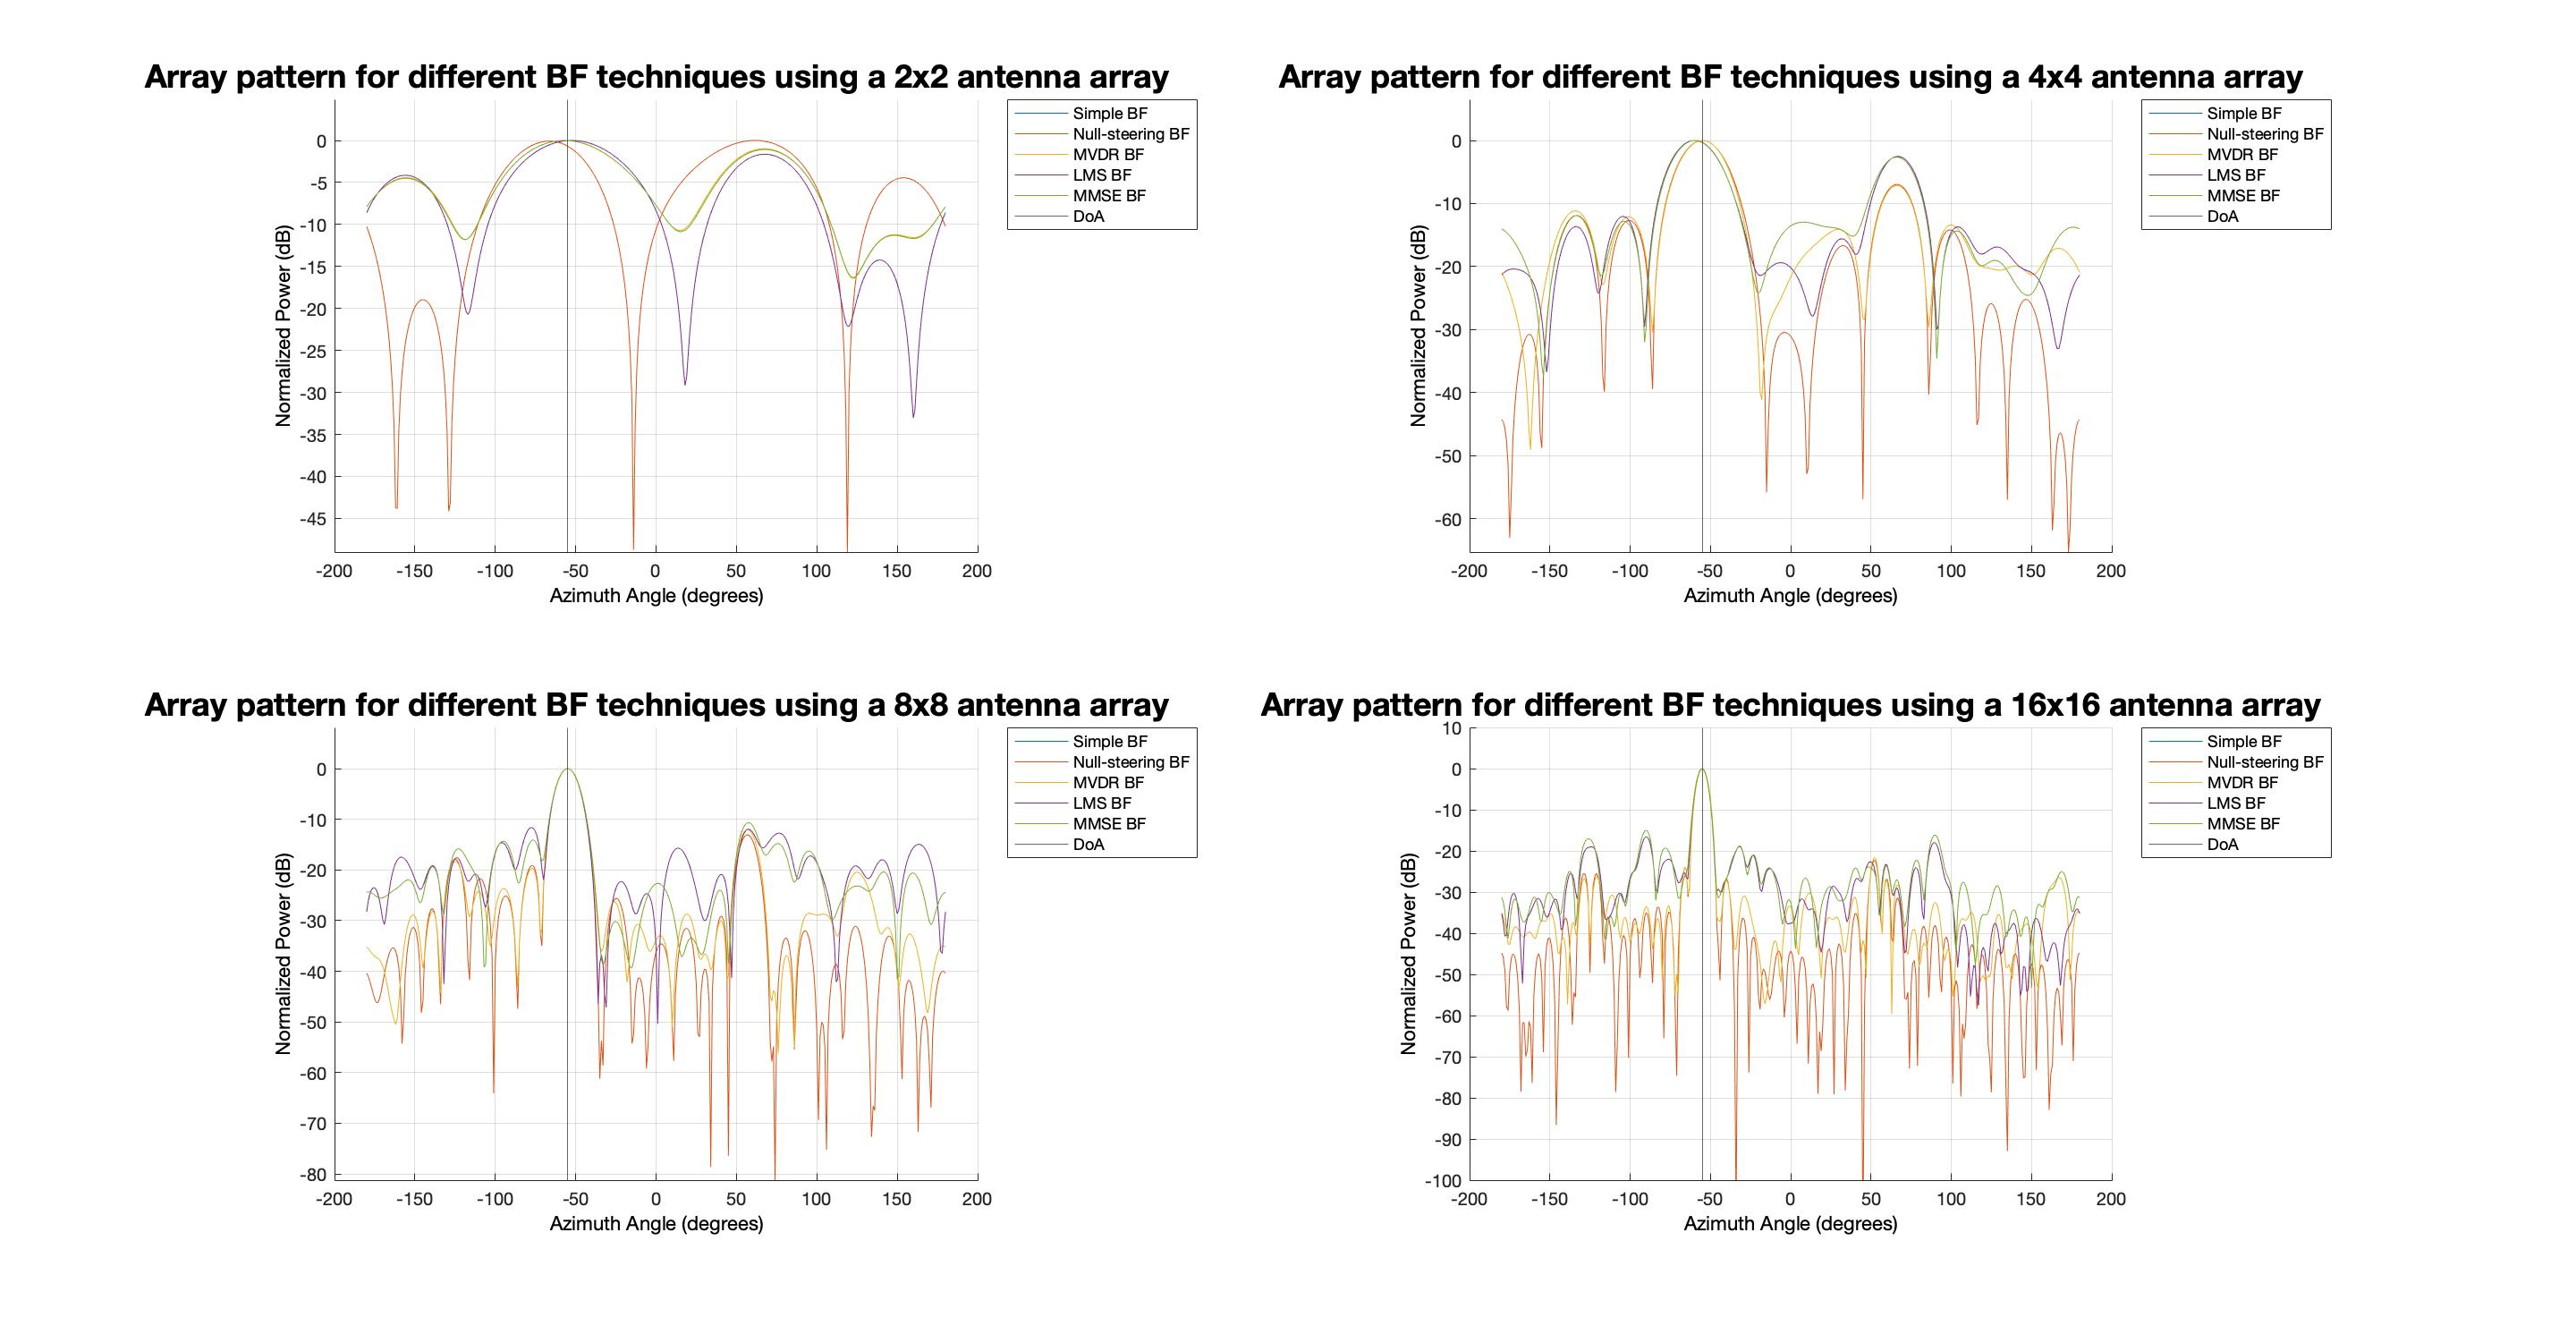
\includegraphics[width=\linewidth]{Array_pattern.jpg}
    \caption{Antenna pattern functions}
    \label{fig:Array_pattern}
\end{figure}

\subsection{Results: \textit{BER}

Finally, the Figure \ref{fig:BER} shows how the $BER$ varies for the five beamformers as a function of the numberr of antennas.\\
As we can see, the $BER$ is different from zero only when we use the 2x2 antenna array. This means that four antennas may not
be sufficient for applying an effective beamforming technique. Actually, this also depends on the beamformer that we are using:
the more it's sophisticated, the less antennas we can use. But this also depends on the specific scenario. \\
What we can in general conclude is that the higher the number of antennas, the lower the $BER$; the actual number of antennas 
needed depends on the target $BER$ and on the model considered.

\begin{figure}[ht]
    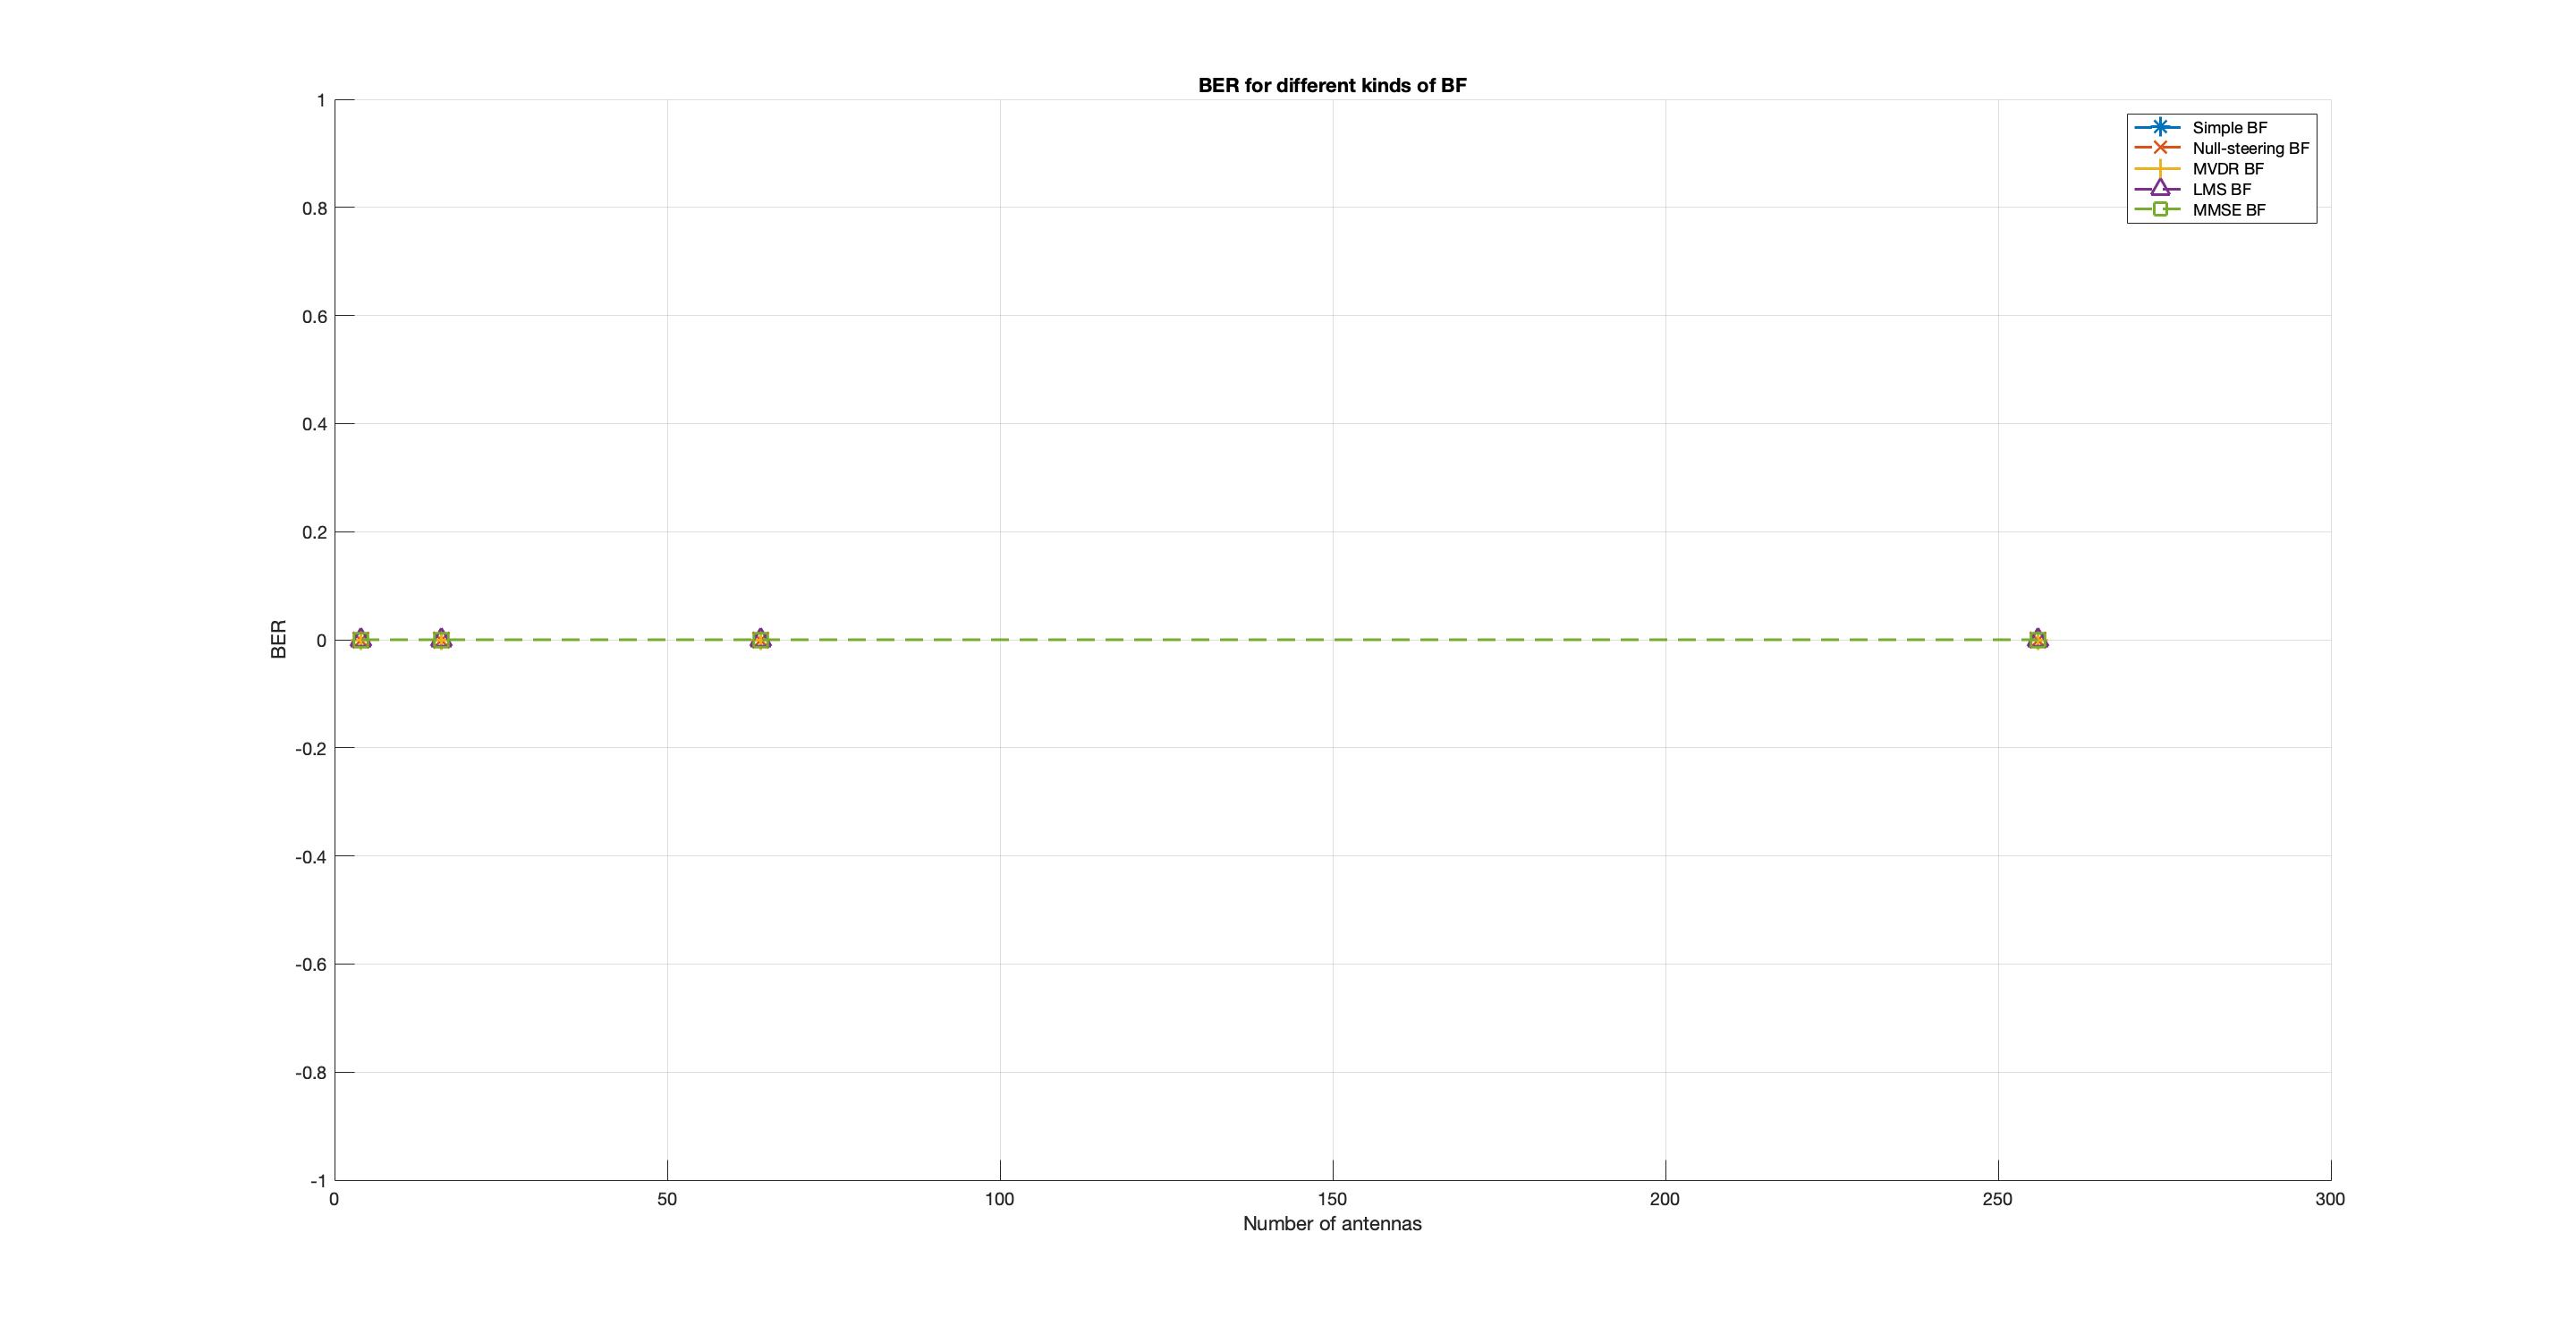
\includegraphics[width=\linewidth]{BER.jpg}
    \caption{BER}
    \label{fig:BER}
\end{figure}

%------------------------------------------------------------------------------------------------------------------------------------------------
\clearpage
\section{Tracking}
\label{sect:project}
In this section, we describe the tracking experiment and all the tecquiques involved.

\subsection{Aim of the Experiment}

The focus of the last part of the Project is to track continuously two vehicles that are moving in a straight line,
and in particular to appreciate the advantages that the LMS beamformer in Frequency domain can offer.

\subsection{Geometry and Paramters}
The two vehicles are moving one towards Nord and one towards Est at 60 $km/h$. The antenna is placed in the origin at a height of 25 meters
and it is equipped with an array of 16x16 Antennas parallel to the ground. The simulation lasts 12 seconds and each vehicle 
exchange 24 packets in total.

This is the Scenario:

\begin{figure}[ht]
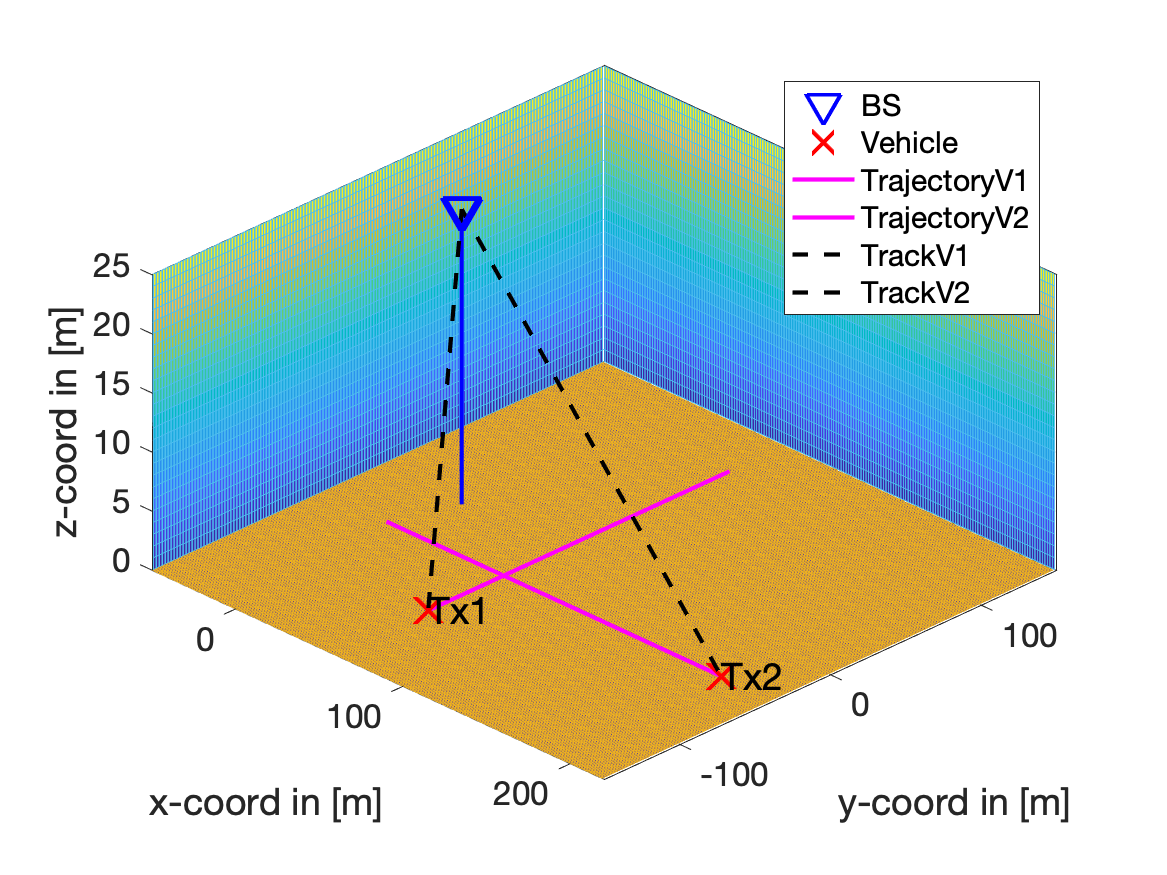
\includegraphics[width=\linewidth]{Quadriga1.png}
  \caption{Scenario.}
  \label{fig:Scenario}
\end{figure}

As parameters we used Carrier Frequency fc = 2.6 $GHz$, OFDM with 4-QAM as modulation with 64 sub-carrier and 100 symbols/packet.

\subsection{Steps of the Simulation}

\begin{enumerate}
    \item \textbf{Generation of the signals} Through the QAM modulator and OFDM modulator. 
    \item \textbf{Creation of the Channel} In this case $QuaDRiGa\_UD2D\_LOS$ channel.
    \item \textbf{Passage of Waveforms in the channel} By means of the convolution with the channel model.
    \item \textbf{Estimation of DoA} With the Music Algorithm.
    \item \textbf{OFDM Demodulation} Applying the FFT on the Signal from each Antenna.
    \item \textbf{LMS Beamformer} For each sub-carrier (In Frequency Domain) using half of the sequence as training.
    \item \textbf{Channel equalization} Applying the Gradient-Descent algorithm to each Sub-Carrier.
    \item \textbf{QAM Demodulation} Finally recovery of the bits and calculation of the BER.
\end{enumerate}


\subsection{Results of the Tracking}

The experiment shows that at the beginning the Tx with Vehicle1 has practically zero errors since it is the nearest to the station
and the music algorithm can estimate without problems its position. Instead the Tx with Vehicle2 has many more errors, due to 
the many multipath of the channel and to the lower received Power.

When they are about the same distance and in normal conditions the track performs without any particular problem.

At the end when Vehicle2 is the nearest to the BaseStation, the situation is inverted and the Tx with Vehicle2 is far more 
reliable that with Vehicle1.

\begin{figure}[ht]
    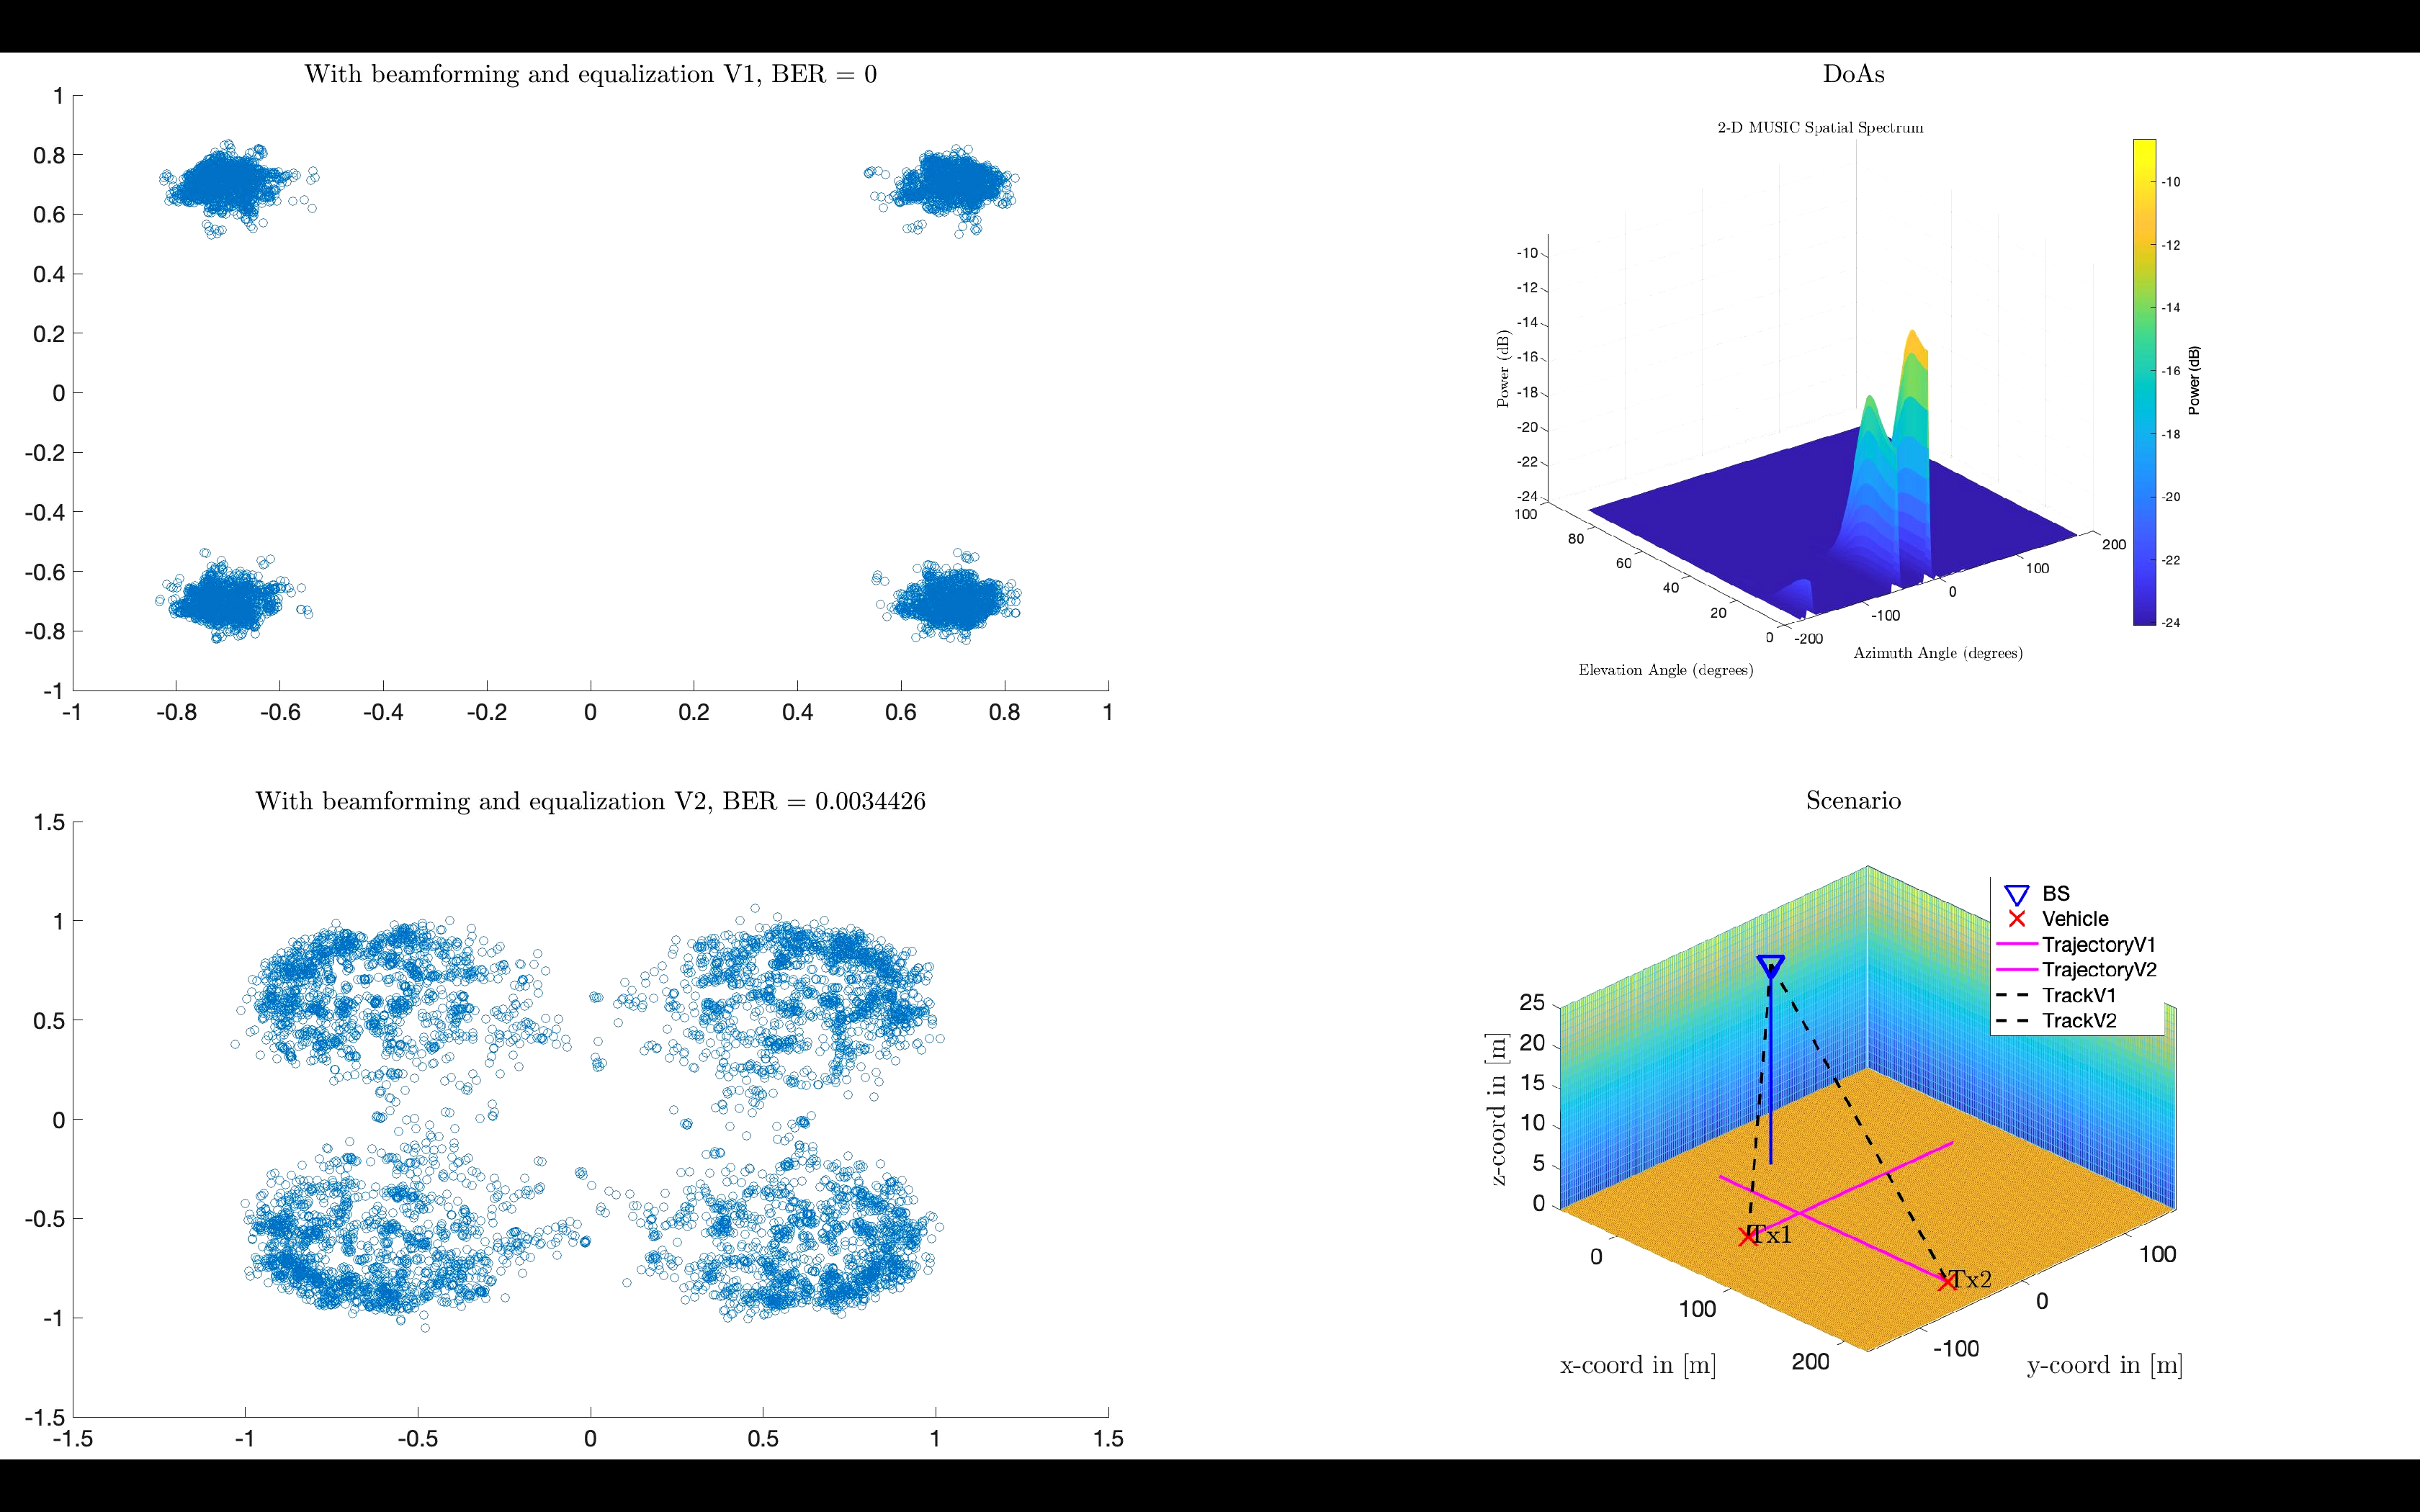
\includegraphics[width=\linewidth]{Begin_tx.png}
      \caption{Beginning of Tx.}
      \label{fig:Begin_tx}
\end{figure}
\begin{figure}[ht]
    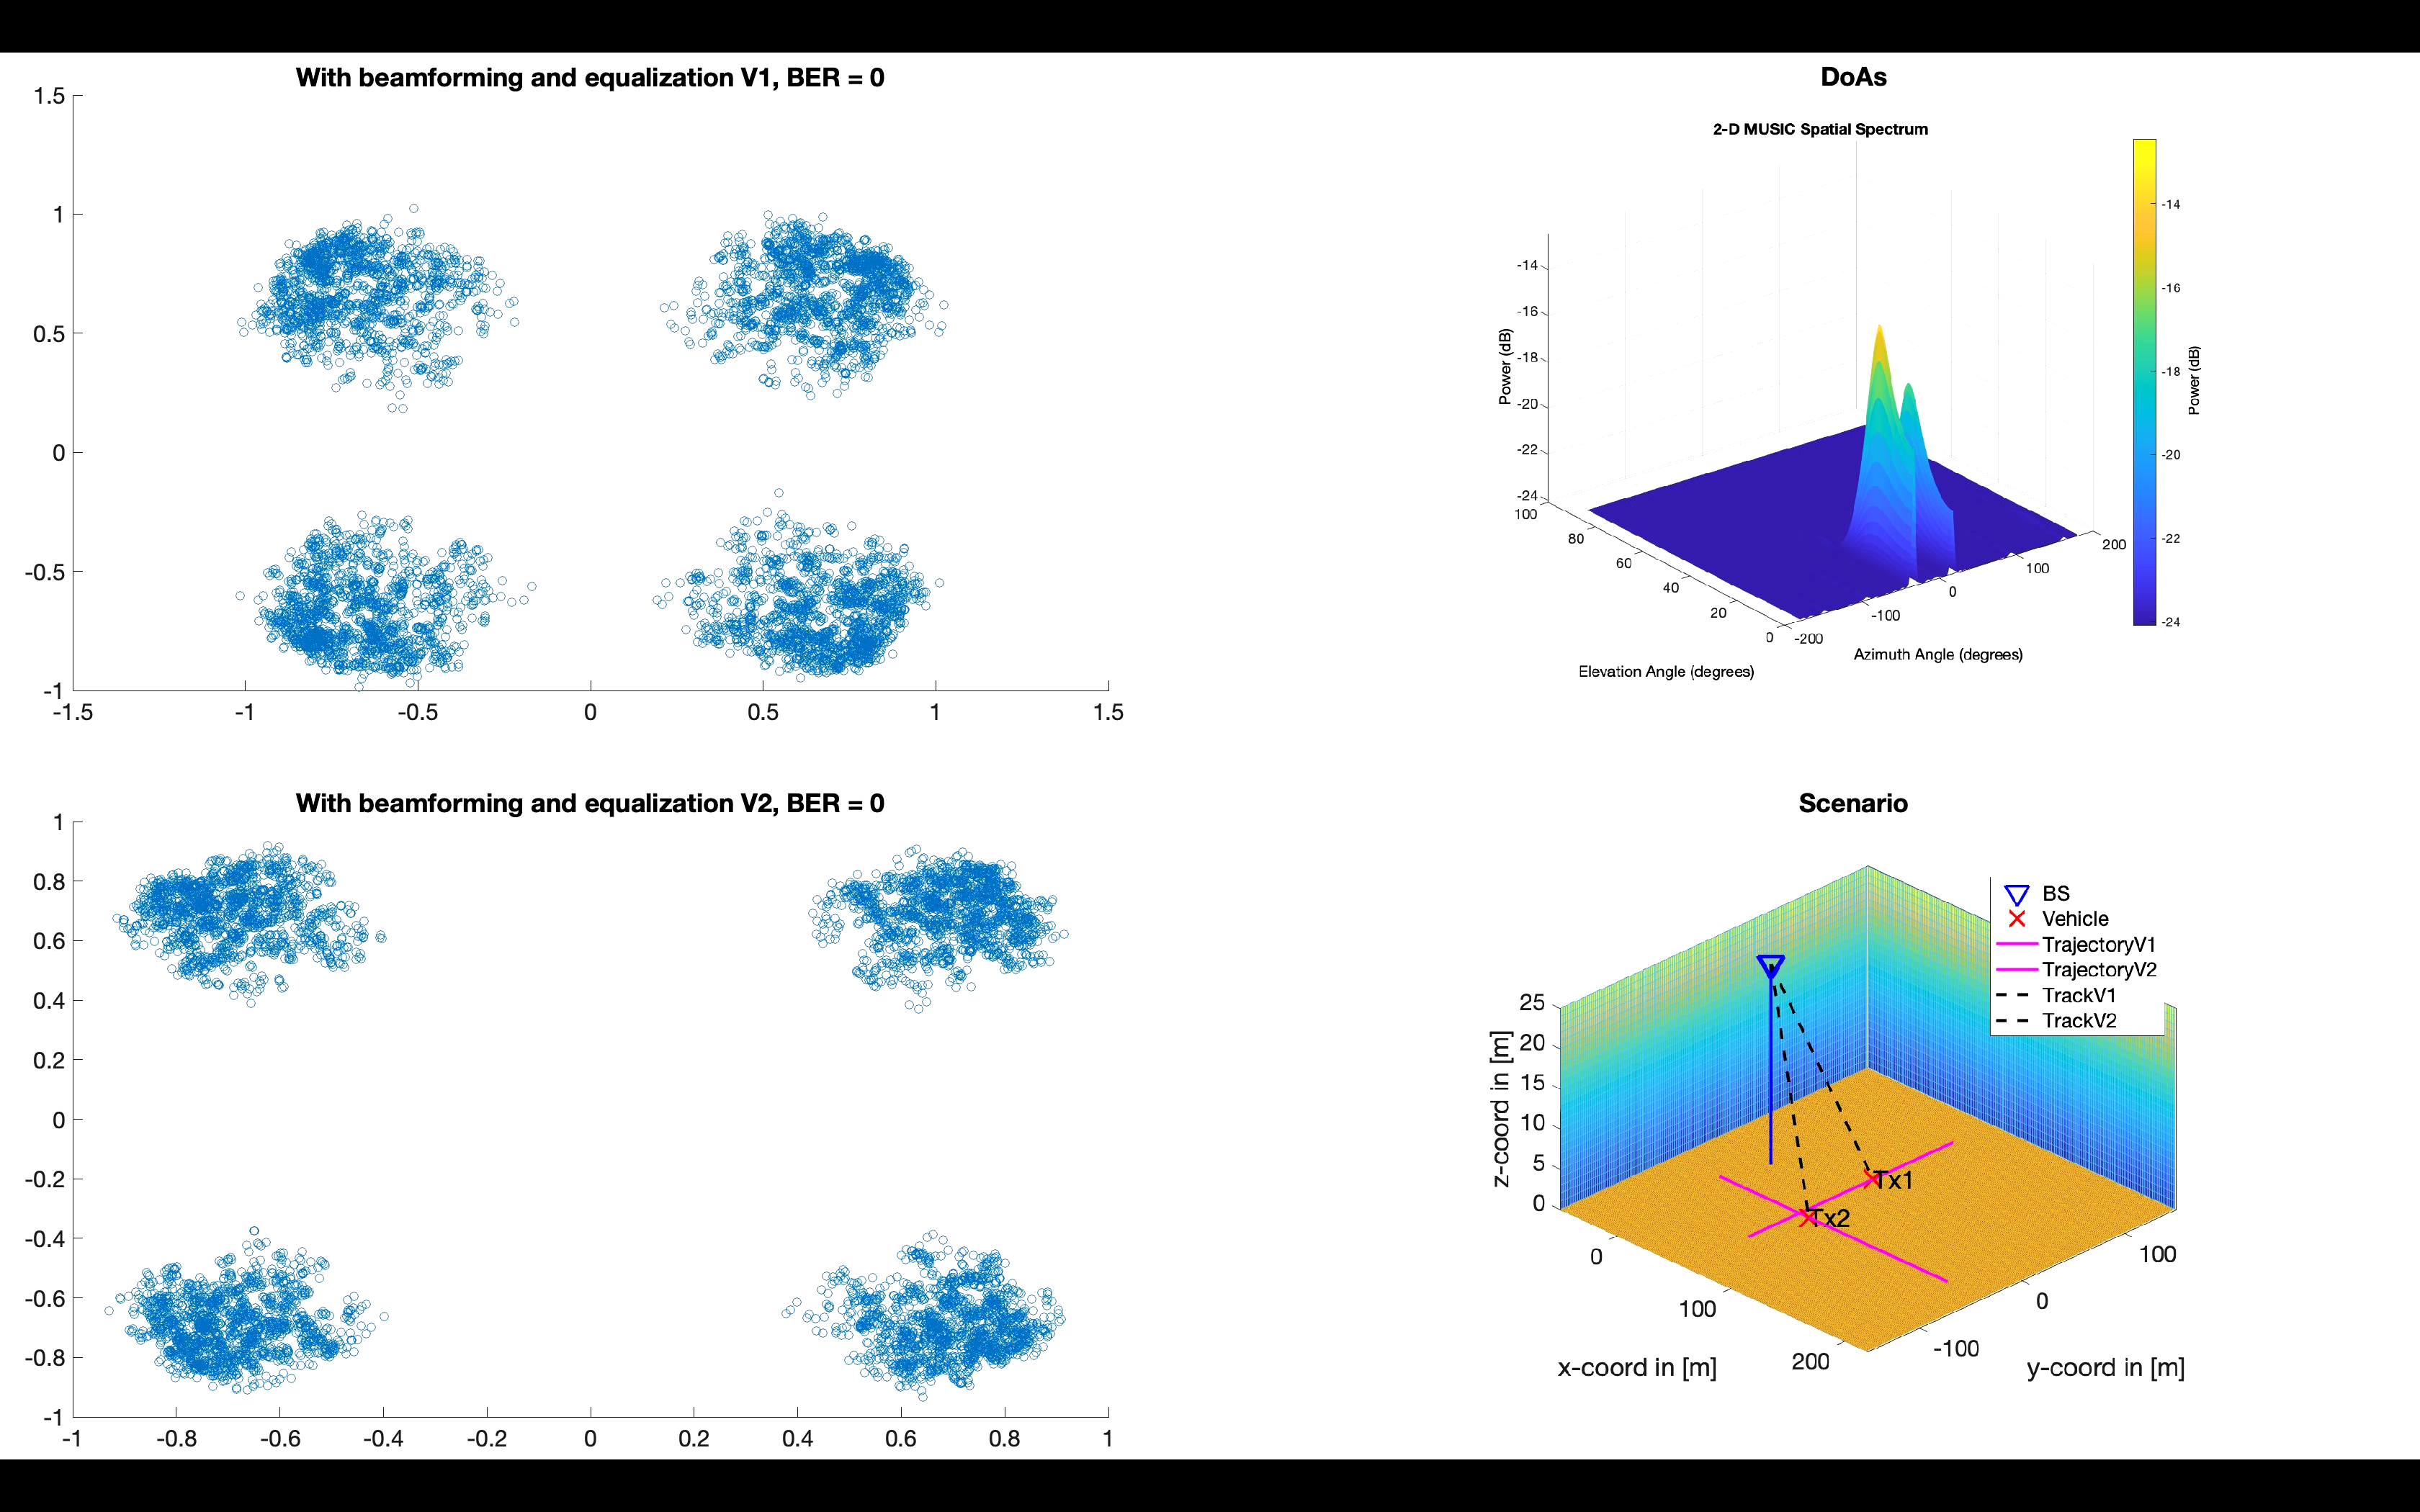
\includegraphics[width=\linewidth]{Middle_tx.png}
      \caption{Middle of Tx.}
      \label{fig:Middle_tx}
\end{figure}
\begin{figure}[ht]
    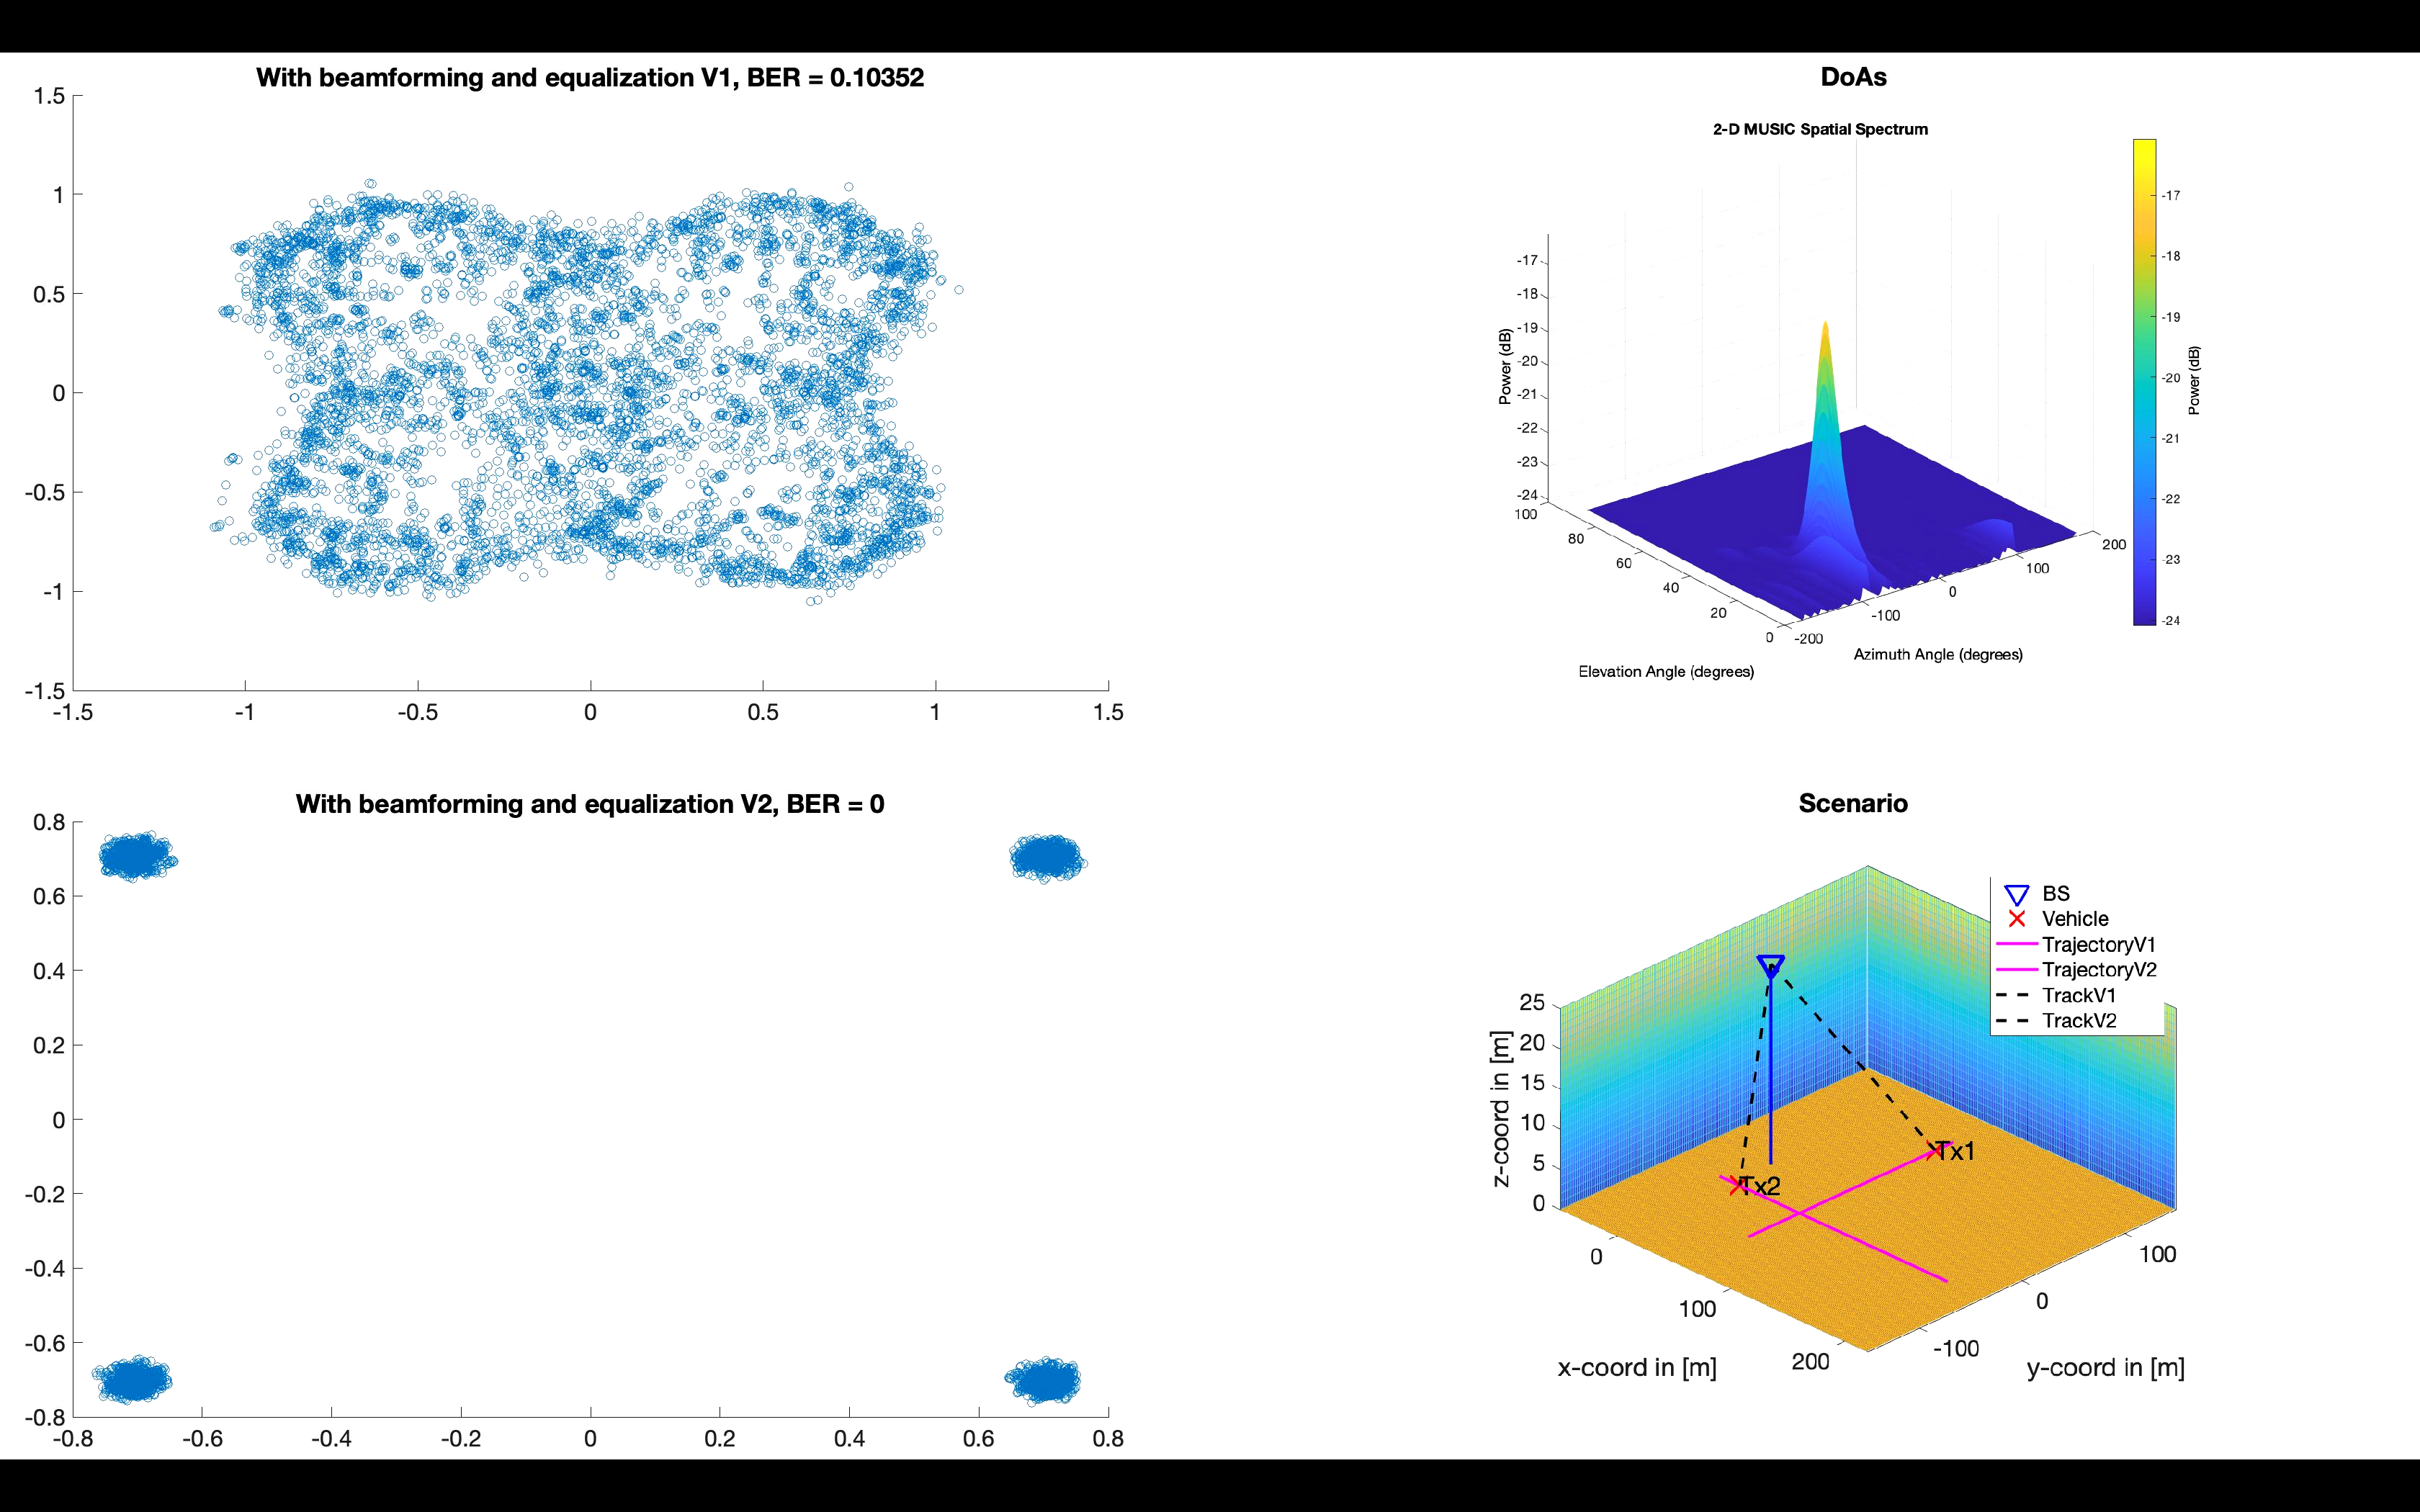
\includegraphics[width=\linewidth]{End_tx.png}
      \caption{End of Tx.}
      \label{fig:End_tx}
\end{figure}


%------------------------------------------------------------------------------------------------------------------------------------------------
\section{Conclusions}
\label{sect:project}
\subsection{What we have learned}

With this project, we have understood the potentials of different techniques of beamforming.\\
We have used beamforming for isolating a source in an enviroment full of interference and for tracking users,
and these two are the main field in which beamforming is used. 

\subsection{Our difficulties}

The core of the project was the implementation of the beamformers and the design of the system for the communication 
between the user(s) and the base station.\\
The main problem we have found was finding the way of implementing digitally the physical formulas and check the physical meaning 
of the results we have obtained.

\subsection{Future developments}

With the new generation of cellular systems, massive MIMO is becoming more and more important.\\ 
With the availability of such a huge number of antennas (for sure, more than 16x16 arrays, which are the biggest we 
have used), beamforming becomes more precise, thus allowing a better localization of sources. 

%------------------------------------------------------------------------------------------------------------------------------------------------
\end{document}